\documentclass[12pt,letterpaper,titlepage]{report}

% packages

\usepackage[final]{pdfpages}
\usepackage[utf8]{inputenc}
\usepackage{mathptmx}
\usepackage{geometry}

% layout

\geometry{
    letterpaper,
    lmargin=0.75in,
    rmargin=0.75in,
    tmargin=1.0in,
    bmargin=1.0in
}

% the real fun begins

\begin{document}

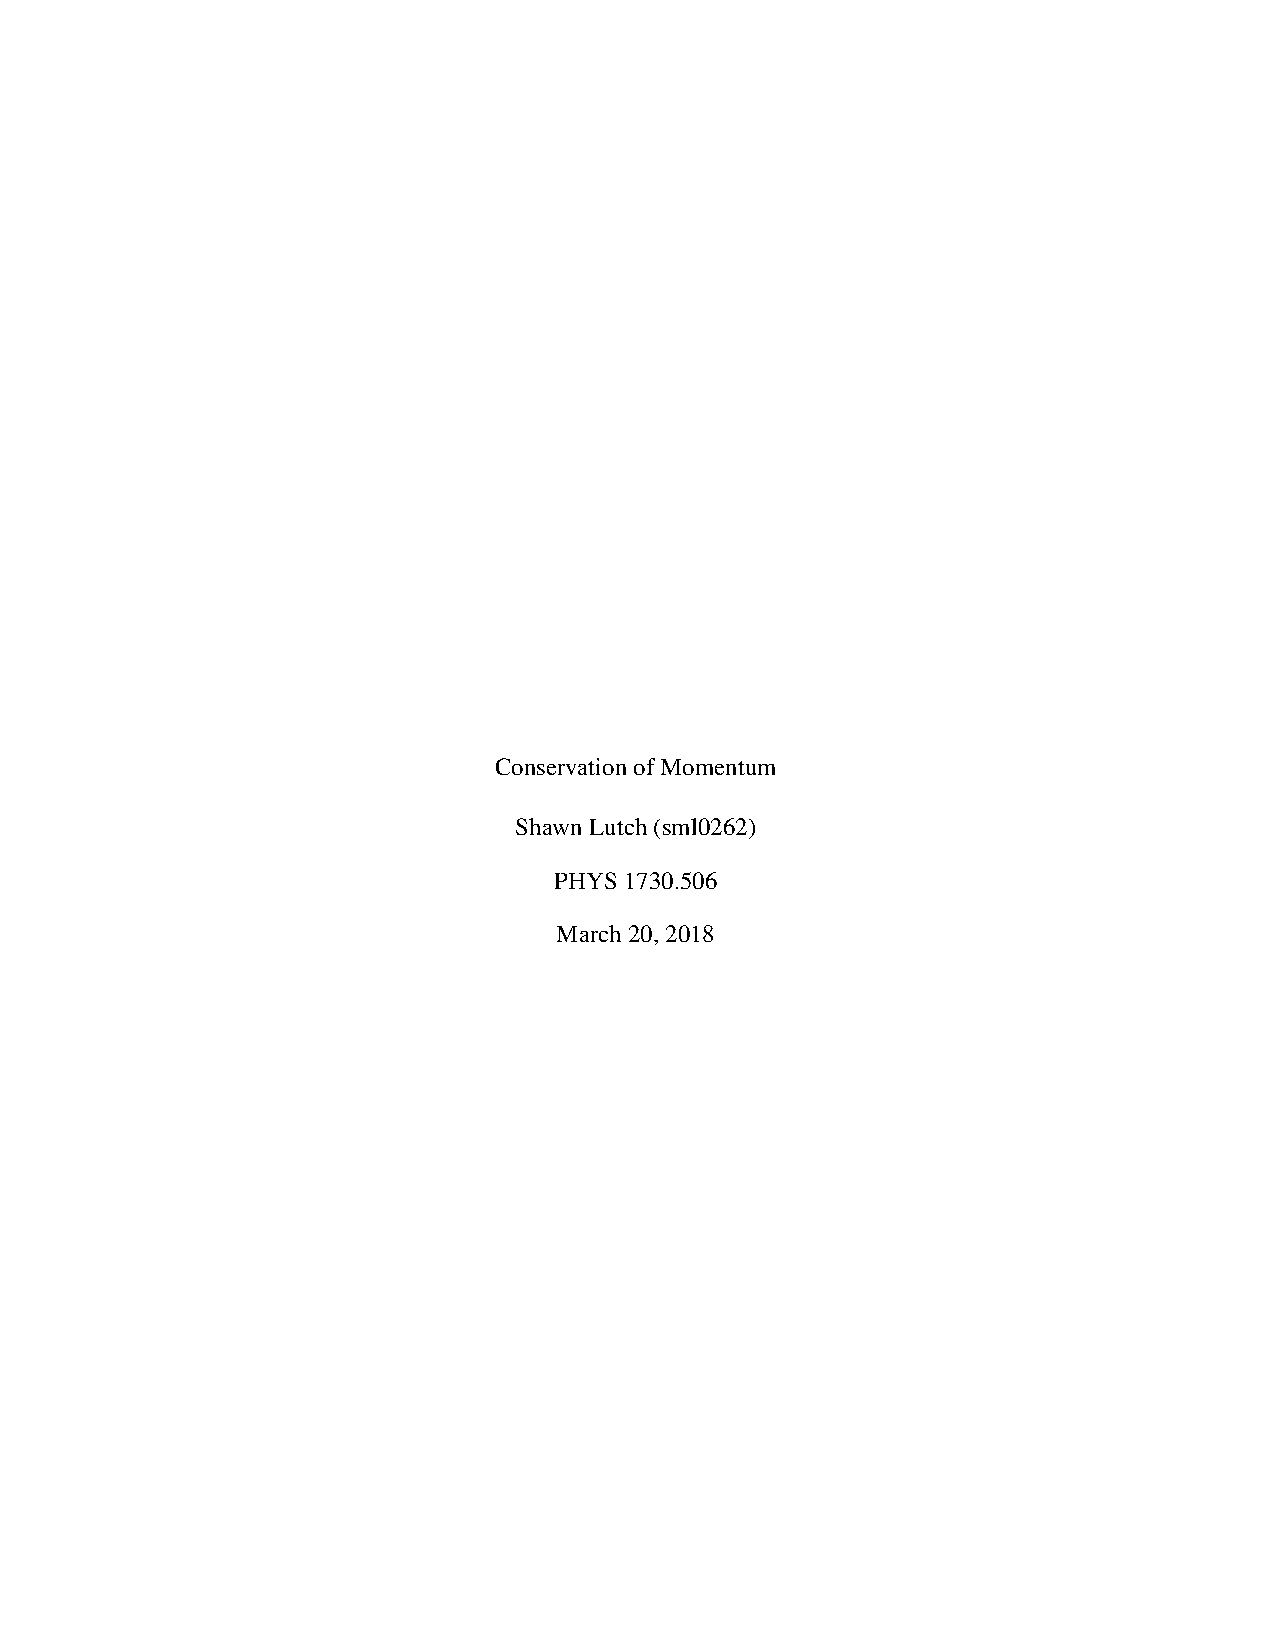
\includepdf{pages/titlepage}

% ABSTRACT

\section*{Abstract}

\noindent
The purpose of this lab is to study conservation of momentum and the 
differences between elastic and inelastic collisions. This lab focuses on
collisions in a one-dimensional system with two objects. By sliding two
gliders with known masses toward each other on an air track and calculating
the total momentum of the system ($p$) and after ($p'$) the collision, we see
that, because $p = p'$, momentum is conserved.

% INTRODUCTION

\section*{Introduction}

\noindent


% APPARATUS

\section*{Apparatus}

\begin{itemize}
    \item Air track
    \item Two gliders
    \item Two photo gates
    \item Computer with timing and analysis software
\end{itemize}

% PROCEDURE

\section*{Procedure}

\noindent
The air track and compressor were set up by the lab instructors prior to
our experiment. We ensured that the track was level by adjusting the base
support screws until a glider in the middle of the track remained stationary.
We then placed a photogate 30 cm from each end of the track and placed a 
rubber band bumper on each end of the track, to prevent the gliders from
colliding harshly into the ends of the track after colliding with one another.

% DATA

\section*{Data}

\begin{tabular}{c || c | c }

\end{tabular}

% CALCS AND GRAPHS

\section*{Calculations and Graphs}

% DISCUSSION

\section*{Discussion of Results and Error Analysis}

% CONCLUSION

\section*{Conclusion}



\end{document}
